% Created 2020-09-28 Mon 16:36
% Intended LaTeX compiler: pdflatex
\documentclass[presentation]{beamer}
\usepackage[utf8]{inputenc}
\usepackage[T1]{fontenc}
\usepackage{graphicx}
\usepackage{grffile}
\usepackage{longtable}
\usepackage{wrapfig}
\usepackage{rotating}
\usepackage[normalem]{ulem}
\usepackage{amsmath}
\usepackage{textcomp}
\usepackage{amssymb}
\usepackage{capt-of}
\usepackage{hyperref}
\usetheme{UoB}
\author{Mark Blyth}
\date{\textit{[2020-09-28 Mon]}}
\title{Intro to programming}
\hypersetup{
 pdfauthor={Mark Blyth},
 pdftitle={Intro to programming},
 pdfkeywords={},
 pdfsubject={},
 pdfcreator={Emacs 27.1 (Org mode 9.3)}, 
 pdflang={English}}
\begin{document}

\maketitle

\section{Presentation}
\label{sec:org7b168b8}
\begin{frame}[<+->][label={sec:org18901f3}]{Aims}
All python-based; no assumed knowledge
\vfill
\begin{itemize}
\item Understand basic principles of computer programming, eg. for communicating with devs
\end{itemize}
\vfill
\begin{itemize}
\item Basic introduction to designing and building short computer programs
\end{itemize}
\vfill
\begin{itemize}
\item Translate "problem statements" into computational algorithms
\end{itemize}
\vfill
\begin{itemize}
\item Provide first steps in computing, to feed into more advanced units later on
\end{itemize}
\end{frame}

\begin{frame}[label={sec:org51ff739}]{Assessment}
\begin{itemize}
\item Syntax test
\end{itemize}
\vfill
\begin{itemize}
\item Caesar cipher project, set end of November
\end{itemize}
\vfill
\begin{itemize}
\item PG TAs mark assignments
\end{itemize}
\end{frame}

\begin{frame}[label={sec:org588aa54}]{Teaching format}
\begin{itemize}
\item Lectures Monday
\begin{itemize}
\item TAs are expected to keep up with these
\end{itemize}
\end{itemize}
\vfill
\begin{itemize}
\item Drop-ins on Wednesday; 10 TAs
\end{itemize}
\vfill
\begin{itemize}
\item 1h tutorials Friday
\begin{itemize}
\item Two sessions 9-10, 1-2, 9 students per group
\item \emph{\alert{Must take attendance}}
\end{itemize}
\end{itemize}
\vfill
Any preferences for drop-ins?
\end{frame}

\begin{frame}[label={sec:org836aa22}]{Your role}
\begin{itemize}
\item Check that students completed, understood weekly exercises
\item Facilitate discussion around approaches, problems encountered
\end{itemize}
\vfill     
Ideas:
\begin{itemize}
\item Pick on students to share their solutions (eg. screen sharing)
\item Build discussion about alternative approaches
\item Make them explain what was hard, any problems they had, how they overcame them
\end{itemize}
\vfill     
Prep: 1 hour watch lecture video/slides, familarisation exercises.
\end{frame}

\begin{frame}[label={sec:orgf822a3f}]{If things go wrong}
\begin{itemize}
\item You should ensure you get to know all your students
\end{itemize}
\vfill     
\begin{itemize}
\item Any that are struggling academically: notify me
\end{itemize}
\vfill     
\begin{itemize}
\item Any that are struggling personally: notify Hemma
\end{itemize}
\end{frame}

\begin{frame}[label={sec:org7059c3b}]{HPT claims}
\begin{enumerate}
\item Email me for approval; break down your hours into
\begin{itemize}
\item Preparation
\item Labs
\item Dropins
\item Marking
\end{itemize}
\item Once approved, submit a claim on MyERP
\item Write in the box "I confirm I have had the authority and confirmation of Mark Blyth on \alert{[date]} that the hours claimed have been completed."
\end{enumerate}

\vfill
Can claim 1.5h preparation time per week
\end{frame}

\begin{frame}[label={sec:org7081a13},plain]{MyERP}
Navigate to MyERP

\begin{center}

\includegraphics[width=.9\linewidth]{./icp_search.png}
\end{center}

\url{https://uob.sharepoint.com/sites/myerp/}
\end{frame}

\begin{frame}[label={sec:orgbd5f742}]{MyERP}
\begin{center}
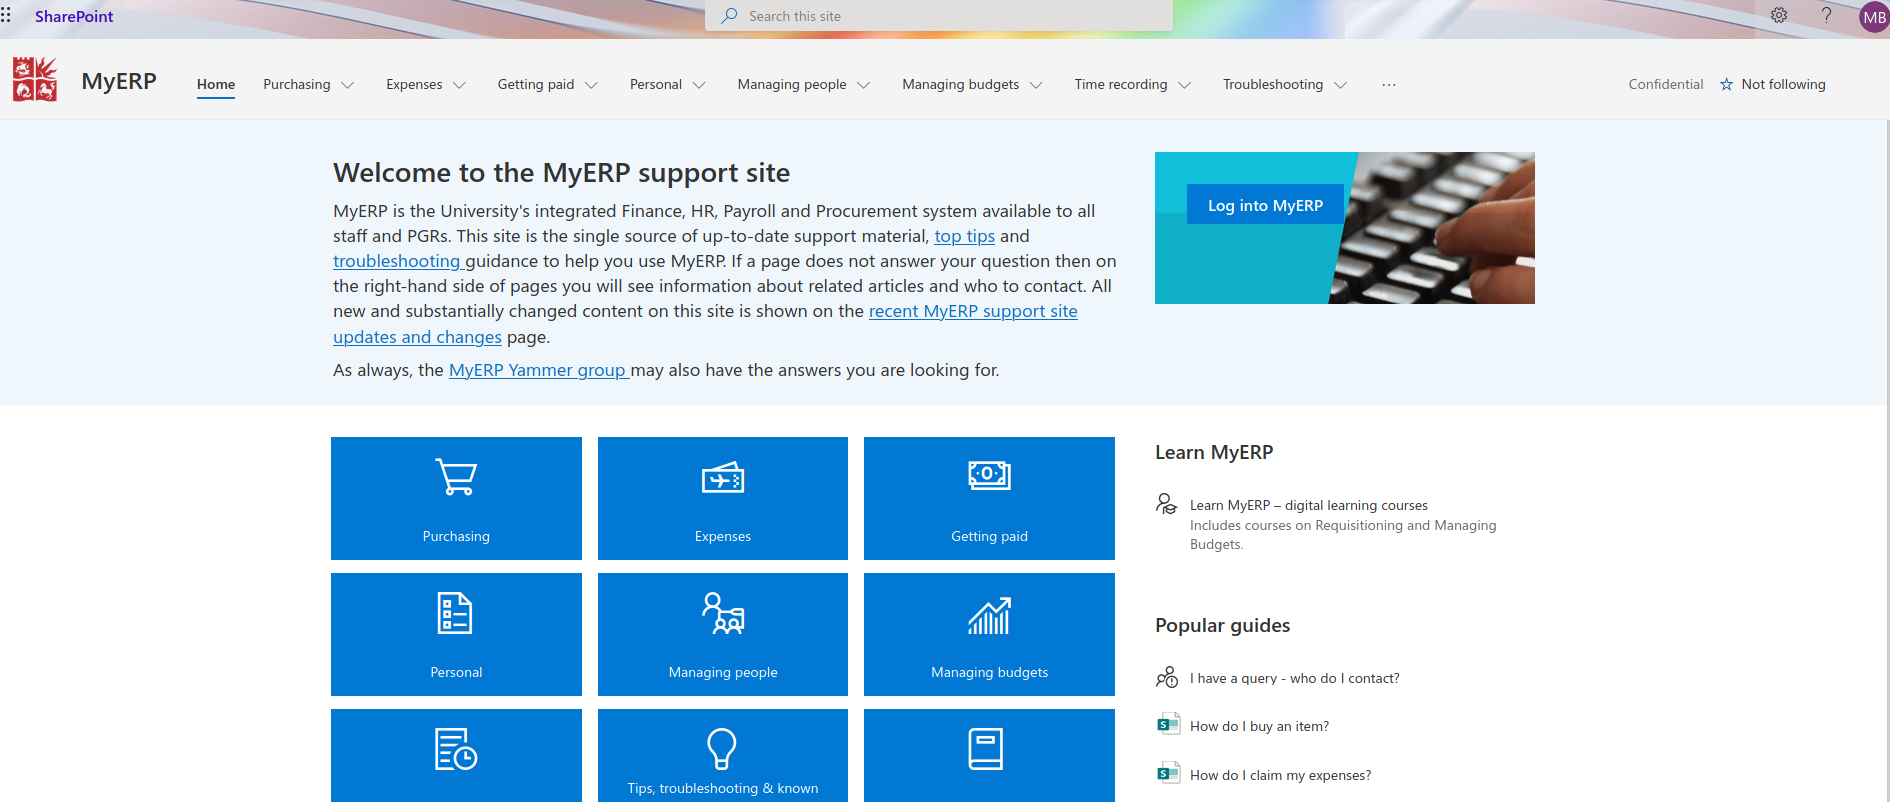
\includegraphics[width=.9\linewidth]{./icp_login.png}
\end{center}
\end{frame}

\begin{frame}[label={sec:orgc7d44f9}]{MyERP}
\begin{center}
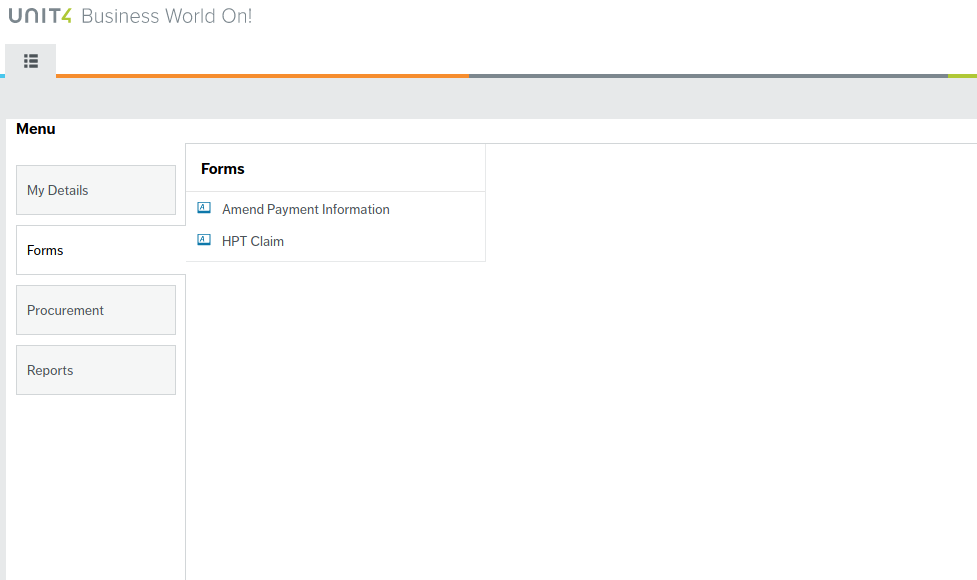
\includegraphics[width=.9\linewidth]{./icp_claim.png}
\end{center}
\end{frame}

\begin{frame}[label={sec:org2c9d7d4}]{Sickness and annual leave}
\begin{itemize}
\item Email me ASAP
\end{itemize}
\vfill
\begin{itemize}
\item Put it on the group calendar
\end{itemize}
\end{frame}

\begin{frame}[label={sec:orgbfc7b1d}]{Questions?}
Slides and an outline document are all available on the icp2020tas sharepoint
\end{frame}
\end{document}
